\documentclass[letterpaper, 11pt]{article} 

\usepackage{graphics,graphicx}
\usepackage{multicol} 
\usepackage{parskip}
\usepackage{amsmath}
\usepackage{multirow}
\usepackage[utf8]{inputenc}
\usepackage{fancyhdr}
\usepackage[title]{appendix}
\usepackage{wasysym}
\usepackage{url}
\usepackage{subcaption}
\usepackage{advdate}

\usepackage[font=footnotesize,labelfont=small]{caption}
\captionsetup{width=0.85\linewidth}

\RequirePackage{geometry}
\geometry{margin=2cm}

\setlength{\parskip}{0.2cm}
\setlength{\parindent}{0pt}

\usepackage{listings}
\usepackage{xcolor}

\definecolor{codegreen}{rgb}{0,0.6,0}
\definecolor{codegray}{rgb}{0.5,0.5,0.5}
\definecolor{codepurple}{rgb}{0.58,0,0.82}
\definecolor{backcolour}{rgb}{0.95,0.95,0.92}

\lstdefinestyle{mystyle}{
	backgroundcolor=\color{backcolour},   
	commentstyle=\color{codegreen},
	keywordstyle=\color{magenta},
	numberstyle=\tiny\color{codegray},
	stringstyle=\color{codepurple},
	basicstyle=\ttfamily\footnotesize,
	breakatwhitespace=false,         
	breaklines=true,                 
	captionpos=b,                    
	keepspaces=true,                 
	numbers=left,                    
	numbersep=5pt,                  
	showspaces=false,                
	showstringspaces=false,
	showtabs=false,                  
	tabsize=2
}

\lstset{style=mystyle}


\title{Assignment 2: Multithreading and Solving System of Linear Equations Algorithms}
\author{
Tai Duc Nguyen \\
ECEC 622: Parallel Computer Architecture
}
\date{\AdvanceDate[-1]\today}

\begin{document}

\maketitle

\rule{\textwidth}{1pt}

\begin{abstract}
	Knowledge from the previous assignment about multithreading's quirks and benefits is leveraged to develop a common algorithm used in solving system of linear equations called Iterative Gaussian Elimination. 
\end{abstract}

\rule{\textwidth}{1pt}

\section{Experimental Setup}

Gaussian Elimination, also known as row reduction, is an algorithm in linear algebra for solving a system of linear equations. It is usually understood as a sequence of operations performed on the corresponding matrix of coefficients. This method can also be used to find the rank of a matrix, to calculate the determinant of a matrix, and to calculate the inverse of an invertible square matrix. 

The multithreaded version of this algorithm is implemented as follows:

\begin{lstlisting}
	Initialize barrier sync
	
	Create threads
	Allocate memory on heap for threads' data
	
	Start all threads. For each thread:
		for k = 0 -> n_rows:
			chunk_size = floor((n_cols-k-1)/num_threads);
			offset = tid*chunk_size + k + 1;
			start = offset;
			if tid < thread_data->num_threads - 1:
				finish = offset + chunk_size;
			else:
				finish = n_cols;
			
			for j = start -> finish:
				A[k,j] /= A[k,k];  // Division
				
			BARRIER SYNC
			
			for i = k + tid + 1 -> n_rows:
				for j = k + 1 -> n_cols:
					A[i,j] -= (A[i,k] * A[k,j]); // Elimination
				A[i,k] = 0;
				i += num_threads; (striding method)

			A[k,k] = 1;
			
			BARRIER SYNC
		
	Stop all threads


\end{lstlisting}

\textit{Note: running \texttt{make all} will generate the report in \texttt{rpt.txt}}

\section{Experimental Result}

\begin{figure}[htb!]
	\centering
	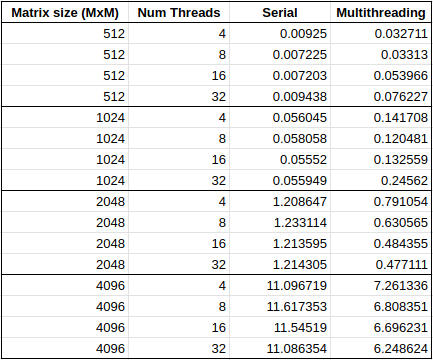
\includegraphics[width=0.6\linewidth]{results.png}
	\caption{Results of execution times in seconds of the serial vs the multithreaded version using the pthread interface}
	\label{fig1}
\end{figure}

\section{Discussion}

From Figure \ref{fig1}, it is apparent that multithreading provides significant improvement only when the problem size is larger than 1024 ($\approx$ 2.4x for 2048, and $\approx$ 2.3x for 4096). In the case where multithreading enhances the program, 32 threads will provide the best speed up. It is not understood yet why the speed up for 4096 is not significantly greater than 2048. This is hypothesized to be the effect of false sharing during the chunking part of the code. Improvements could be made to convert that part into striding instead.

\end{document}